% format two pieces of text, one left aligned and one right aligned
\newcommand{\headerrow}[3] {
\item[] #1 \hfill #3}
%
\newenvironment{position}{
  \begin{itemize}[leftmargin=*]
    \setlength{\itemsep}{1pt}
    \setlength{\parskip}{0pt}
    \setlength{\parsep}{0pt}
}{\end{itemize}}

\section{Experience}

\subsubsection{Sharecare, Inc.}

\begin{position}
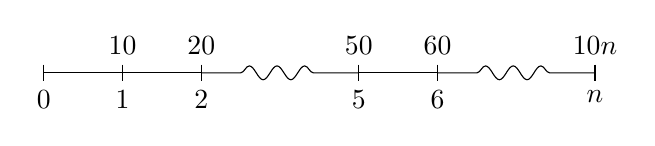
\begin{tikzpicture}
%draw horizontal line
\draw (0,0) -- (2,0);
\draw[decorate,decoration={snake,pre length=5mm, post length=5mm}] (2,0) -- (4,0);
\draw (4,0) -- (5,0);
\draw[decorate,decoration={snake,pre length=5mm, post length=5mm}] (5,0) -- (7,0);

%draw vertical lines
\foreach \x in {0,1,2,4,5,7}
\draw (\x cm,3pt) -- (\x cm,-3pt);

%draw nodes
\draw (0,0) node[below=3pt] {$ 0 $} node[above=3pt] {$   $};
\draw (1,0) node[below=3pt] {$ 1 $} node[above=3pt] {$ 10 $};
\draw (2,0) node[below=3pt] {$ 2 $} node[above=3pt] {$ 20 $};
\draw (3,0) node[below=3pt] {$  $} node[above=3pt] {$  $};
\draw (4,0) node[below=3pt] {$ 5 $} node[above=3pt] {$ 50 $};
\draw (5,0) node[below=3pt] {$ 6 $} node[above=3pt] {$ 60 $};
\draw (6,0) node[below=3pt] {$  $} node[above=3pt] {$  $};
\draw (7,0) node[below=3pt] {$ n $} node[above=3pt] {$ 10n $};
\end{tikzpicture}

  %% \headerrow{QA Architect}{Sharecare, Inc.}{Aug 2012 - Present}
  %% \headerrow{Build Manager}{Sharecare, Inc.}{Oct 2011 - Aug 2012}
  %% \headerrow{QA Engineer I}{Sharecare, Inc.}{Aug 2011 - Oct 2011}

  \paragraph{Honeydew:} Perl, PHP/jQuery/DHTMLX, Saucelabs, Webdriver
  \begin{myitem}
  \item Developed an in-house Cucumber analog, building a full fledged cross-browser automation suite
  \item Rewrote the backend to update the project from Selenium RC to Webdriver
  \item Added monitoring system to alert when critical production functionality tests failed
  %% \item Interprets DSL feature files and executes them locally or on Saucelabs' entire browser suite, recording
  %%   the video with subtitles of each step execution
  \item Enhanced front end with autosuggests, instant feature file searching, per-user default
    settings, and general widespread usability improvements
  \end{myitem}
%
  %% (setq tex-main-file "c:/daniel/resume/resume.tex")
%
  \paragraph{Squash:} Perl, MySQL
  \begin{myitem}
  \item Wrote a site crawler checks headers on URLs and all resources embedded from a sitemap
  \item Scanned three production websites, over 1.5 million pages,
    each night, producing daily email reports
  %% \item Stored all data in a DB for trend analysis (comparing builds, or the performance of a single
  %%   page over time)
  \end{myitem}
%
  \paragraph{REST API:} Perl, PHP/jQuery, MongoDB
  \begin{myitem}
  \item Built a test suite with SPORE to test our internal REST APIs
  \item Created a UI where other QA engineers can execute project tests
  \end{myitem}
%
  \paragraph{Manual QA Testing:} JIRA
  \begin{myitem}
  \item Routinely performed manual browser tests in all major browsers,
  \item Tested stories and documented bugs in JIRA with extensive screenshot and video evidence
  %% \item Frequently debugged complicated issues alongside developers
  \end{myitem}
\end{position}
